\documentclass[sigconf]{acmart}
\usepackage[T1]{fontenc}
\usepackage{lipsum}
\usepackage{csquotes}
\usepackage{listings}

\def\BibTeX{{\rm B\kern-.05em{\sc i\kern-.025em b}\kern-.08emT\kern-.1667em\lower.7ex\hbox{E}\kern-.125emX}}

\setcopyright{none}

\settopmatter{printacmref=false}
\renewcommand\footnotetextcopyrightpermission[1]{} 
\pagestyle{plain} 
\begin{document}

\title{Prediction of Citable Articles in World Trade Organization Using Deep Learning} 

\author{}
\thanks{All reproducible codes are publicly available at \hyperlink{https://github.com/syyunn/DeepWTO}{https://github.com/syyunn/DeepWTO}}
\orcid{0000-0002-4544-8461}
\affiliation{
    \institution{}
    \position{}
    \email{}
    }

\begin{abstract}

 Recent development of Artificial Intelligence (AI) with deep learning has been incredibly successful. However, application of those successful AI techniques into legal field has been relatively contemned. Therefore this research had chosen one of the most successful legal systems, World Trade Organization (WTO), to apply deep learning techniques to predict which legal articles of WTO could be cited for each different problematic government measure. 
 
 Since preparation of accurately labelled dataset is vital to successful train of neural network, this research prepares a labelled dataset with regards to which legal articles of WTO have been cited for a problematic government measure throughout the entire history of WTO dispute settlements. 
 
 With the prepared dataset, we had trained the neural network with structure in Fig \ref{fig:teaser} and evaluated the classification power of the trained model with AUC-ROC (Area Under the Curve of Receiver operating characteristic) metric.
 \end{abstract}

\keywords{Artificial Intelligence, Natural Language Processing, Legal NLP, Computational Law}


\begin{teaserfigure}
  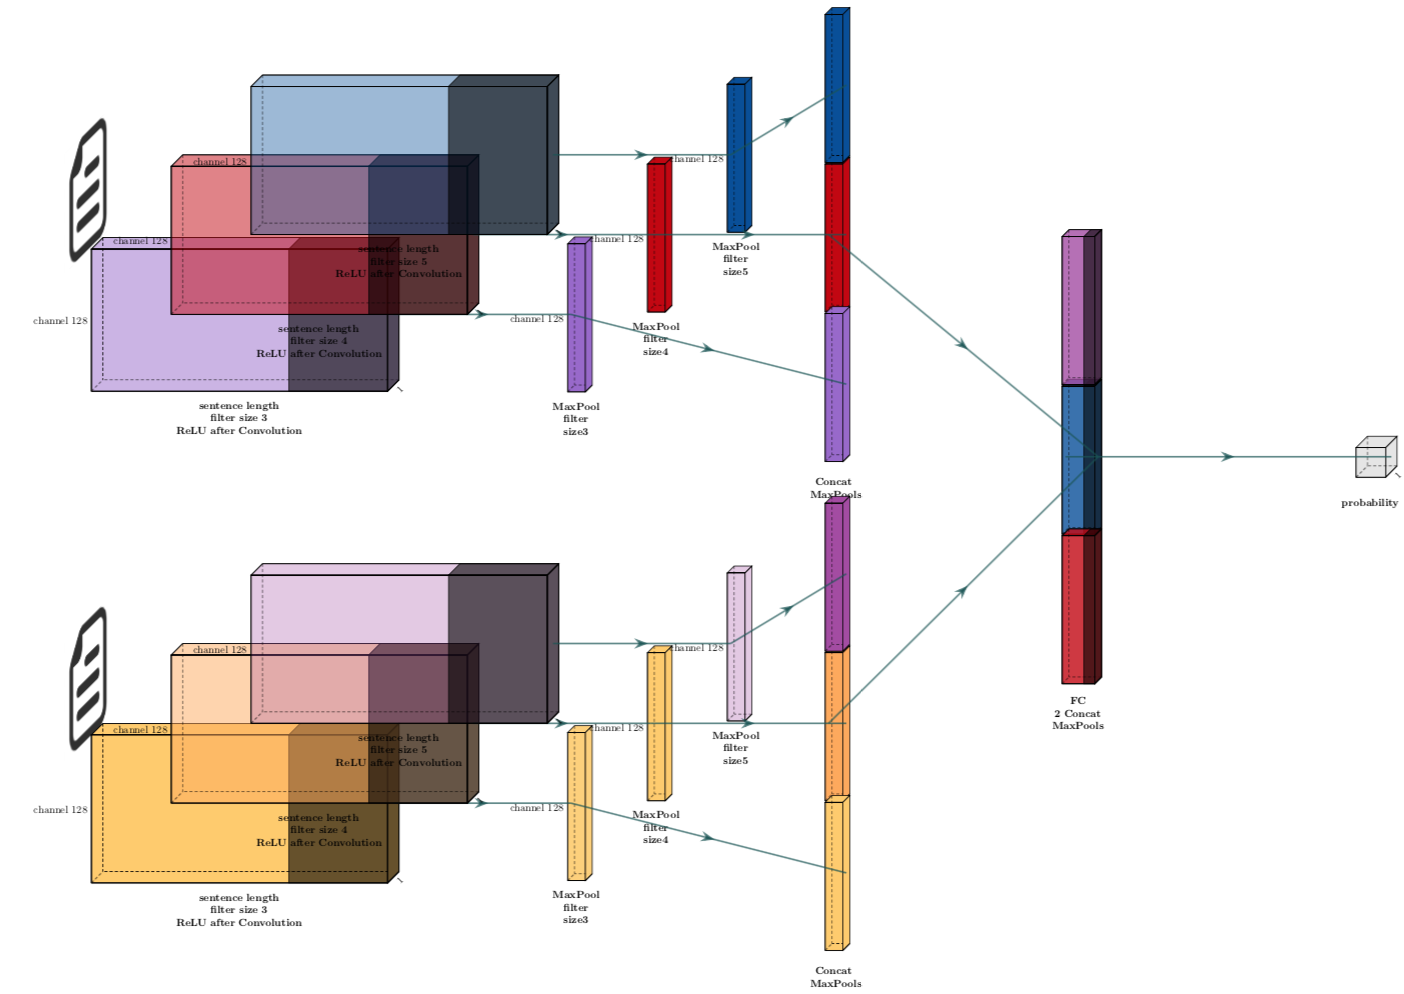
\includegraphics[width=\textwidth]{network.png}
  \caption{TextCNN \& Legal Reasoning Network}
  \Description{the network used in the paper.}
  \label{fig:teaser}
\end{teaserfigure}

% This command processes the author and affiliation and title information and builds
% the first part of the formatted document.
\maketitle

\section{Introduction}
After the novel experimental approach to transfer the words-relations into metric space (Word2Vec)  \cite{DBLP:journals/corr/MikolovSCCD13}, there has been a significant advancement of Natural Language Processing (NLP) combined with deep learning. The advancement was due to the finding of effective method regarding how to represent human words into a form that artificial neural network can compute and understand. 

After the successful implementation of those advancement into public service such as \textit{Google Translator}, NLP related tasks - such as document classification and text generation - combined with several commercial domains - such as spam filtering, review classification and composing lyrics have successfully come into our life and are working around as a commercial service. 

However, specifically in the fields of law, any commercial service or product designed with deep learning has not been released or proven its usefulness to the public. This scarcity of implementation of AI techniques to legal fields is generally due to the lack of available public dataset. Since deep learning is to learn how to map a set of data points into another domain with lots of data, this lack of data has limited the research chance of deep learning in the field of law.

Moreover, law itself is essentially local and requires high-level of expert knowledge to understand. If one compares this localness and experteness with how deep learning has evolved, it's pretty much understandable why the legal AI has not been developed as much as other research field, such as computer vision. The canonical process of how deep learning develops is centered with  verified and well constructed datasets, such as MNIST (hand-writeen digits), MS-COCO (image segmentation) and ImageNet (object detection) attended by the lots of collaborative research in global level. Those dataset is easily verifiable because it does not require any domain-specific knowledge and it's all written in English. Upon this research-friendly ground, collective members of deep learning society has constructed and experimented several variants of neural network to publicly open and shared dataset and it has led the fast development of deep learning in such domain.

So far, however, there's no publicly known dataset with which the research community can indulge together in legal field. As mentioned earlier, the localness of legal fields and its requirements of expert knowledge has limited its possible development and chance of collaborative development of deep learning in this field. Therefore, this research has focused on to provide ready-to-use dataset in legal field. Considering about how to overcome the general localness of legal field, the research had chosen the WTO legal system, which is one of the most successful international legal systems operating in English. Since the WTO official websites provides which provisions of WTO legal texts has been cited for each different dispute between countries, the research crawls the data from the web and processed those into easily feedable format, json, and published the dataset on the \textit{GoogleDrive \footnote{https://drive.google.com/drive/folders/1BpwYLqSBXxSgv8cmItwbohIkfebJr3lX?usp=sharing}}. How those dataset has been processed and organized with which structure will be explained in section 3.

The dataset is targeted on the one class True or False
classification problem. Since the WTO provides a chance of complaining with regards to a government's possible illegal action which is contrary to spirit of free-trade, there exists a different combination of legal articles that is applicable to each different case of government action. Therefore, this research has construced a paired dataset, where each pair consists of cited legal articles and text decription of problematic government action. 


Moreover, as a main contribution, the research has found how the textual content of legal provision helps neural network to enhance its capability to predict the citability of each article for each different situation in accurate manner. Those accuracy is all measured by AUC-ROC curve, which is one of the standard metrics to measure the accuracy of classification model. The model that is trained in this study achieved 0.85 of AUC-ROC, which is way bigger than the naive-baseline of 0.5. This means that the model actually successfully learned about how to distinguish whether a legal article is applicable or not to given government action description.\vspace{0.5mm}

In summary, this research has the following main contributions: \vspace{2mm}

\textbullet \hspace{1mm}  Provides publicly accessible dataset with which anyone can use to experiment their own deep learning model in relatively data scarce legal domain.\vspace{2mm}

\textbullet \hspace{1mm} Proves the possibility that deep learning can learn and understand legal reasoning so that it can predict which articles of WTO legal texts could be cited for each different legal situation.\vspace{2mm}

\textbullet \hspace{1mm} Proves that contents of legal articles enhances model's capability to learn and understand the given legal contexts which leads to the enhancement of classification power likewise as human does.

\section{Related Works}
This research falls into the category of one class True or False classification problem in terms of the problem setting. In addition, this research falls into the study of Deep Learning (DL) in terms of the methodology since this research has adopted DL as a main tool to solve the problem. Moreover, this research falls in to the Natural Language Processing (NLP) in terms of data attribute since the research deals with the textual data as an input. This section will introduce important literatures that is relevant to each category of this research. \\\\
\textbf{Word Embedding} As mentioned in introduction, it is required to transform a human word into numerical vector before we let the computer to analyze human language. This transformation technique had been introduced first in \cite{DBLP:journals/corr/MikolovSCCD13}, and later the transformation has not just been limited to word level but has been narrowed down to character level to handle the situation of misspelling or named-entity recognition problem more robustly \cite{DBLP:journals/corr/KimJSR15}. Those transformations later got to be called Word2Vec, Char2Vec respectively. This transformation is formally called "embedding (into metric space)" since after the transformation, each pair of numerical vectors that are corresponding to each word or character retains their own distance and it fits into definition of the metric space in mathematics. Mathematically, mapping the elements into the metric space is called "embedding" and a visible representation of the result of embedding is illustratively shown in Figure \ref{word2vecFig}. 
\begin{figure}
  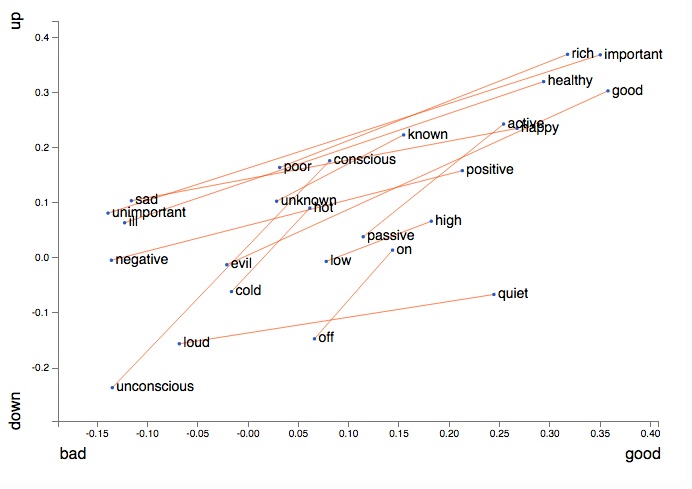
\includegraphics[width=\linewidth]{word2vec2D.png}
  \caption{Word2Vec Example :  Projection Into 2D Space \cite{word2vec}}
  \label{word2vecFig}
\end{figure}
\\\\
\textbf{Document Classification} In NLP, after the embedding of words, those numerical vectors gets to be fed into the neural network to perform specific tasks. As mentioned in introduction, this research premises the one class True or False classification as its problem setting and the classification problem in NLP is generally researched under the name of "document classification". 
Document is defined as a "list of words in sequence" and each documents gets its own label class(es). For example, under the class class name of "sentiment", "positive" or "negative" label exists in IMDB movie review dataset \cite{maas-EtAl:2011:ACL-HLT2011}. Since the document in each domain retains its own unique structure and hierarchy to comprise its own meaning and information, cost effective network structure that can learn those structure and hierarchy is the key research interest in document classfication. Currently most famous and known-to-be well working network structures are BERT \cite{DBLP:journals/corr/abs-1810-04805}, Self-Attention \cite{DBLP:journals/corr/VaswaniSPUJGKP17}, TextCNN \cite{DBLP:journals/corr/Kim14f} and its variants. Detailed explanation about each specific network structure might be a bit of deviation from this research purpose, so it's omitted but the relevant network that this research has been referred will be explained later in section 4.1.
\\\\
\textbf{Evaluation Metric} After the selection of model and train the neural network, one needs to evaluate the trained model to determine whether the training was successful or not. This research adopts AUC-ROC\cite{Bradely1997} as its evaluation metric, which tells about how much the trained model is capable of distinguishing between labels in class. The benefit of using AUC-ROC as classifciation model has been well summarized in \cite{Bradely1997} as following:\\\\\indent \textbullet \hspace{1mm}  It is independent of a decision threshold chosen.\\\indent \textbullet \hspace{1mm}  It gives an indication of how well separated the
negative and positive classes are for each decision threshold.\\

Since this research aims to solve one class True/False classification, the AUC-ROC metric can provide an intuitive explanation about how much the model becomes to hold its classification power as a result of training regardless of specific threshold criterion.\\

In other words, AUC-ROC provides a kind of bird-eye view to the classification model whether it's well-trained or not with all possible threshold criteria considered.

\section{Data Preparation\protect\footnote{\MakeLowercase{All codes that is used for preparation of the data is available at \url{https://github.com/syyunn/DeepWTO/tree/master/prep}}}}
\subsection{Components of Data}

Basically, the WTO legal process determines whether a country's government measure at issue is consistent to a certain article(s) of WTO legal provisions. For example, in case a country's government measure is inconsistent with the WTO legal article, the ruling body of WTO denotes as following which is cited from the panel report of \textit{Korea Chilled Beef Case}:
\\
\begin{displayquote}{ "Korea\textquotesingle s domestic support for beef in 1997 and 1998 exceeded the de minimis level contrary to Article 6 of the Agreement on Agriculture."\\ 
\end{displayquote} The case \textit{Korea Chilled Beef} is complained by the US government in respect of a regulatory scheme of South Korea government that allegedly discriminates against imported beef. The United States has complained the problematic regulatory scheme of Korean government with following legal articles of WTO:\\
\begin{displayquote}
    Agreement of Agriculture: Art.3, 4, 6, 7\\
    GATT 1994: Art. II, III, X, XI, XVII\\
    Import Licensing: Art. 1, 3\\
\end{displayquote} As the above quote from the panel report of \textit{Korea Chilled Beef Case} has denoted, Korea's domestic support has been determined as an inconsistent action to the article 6 of Agreement on Agriculture. As shown with the example of \textit{Korea Chilled Beef Case}, for each case, WTO official websites provides two different kinds of information - the first one is about the short textual summary about which government measure has become the issue at the case (so called "Factual Aspect") and the second one is about which legal articles of WTO has been cited for the case (so called "Articles Cited").  

This research has gathered every two information - \textit{Factual Aspect} and \textit{Articles Cited}- for each case from the WTO official websites and parsed those information. Then store the data in format of \textit{json}, which is an open-standard file format that uses human-readable text consisting of key-value pairs. The data is published on \textit{Google Drive}\footnote{\url{https://drive.google.com/drive/folders/1BpwYLqSBXxSgv8cmItwbohIkfebJr3lX?usp=sharing}}. 

\subsection{Detailed Data Specification}
Current version of dataset consists of 11,440 data that shares the following format of key-value pairs:\\
\begin{displayquote}
\noindent\rule{7cm}{0.4pt}
\textbf{Shared Data Structure}\\\\
 \{"id": dispute settlement number\_ article number, \\
   "gov": textual description of government measure, \\
   "art": article contents that corresponds to the article number\\ 
   "label": [0] if not cited, [1] if cited\}\\   
\noindent\rule{7cm}{0.4pt}
\textbf{Example from \textit{Korea-Beef Case}}\\\\
    \{"id": DS161\_Article III:4, \\
   "gov": "Korea", "Government", "banned", "importation", "from", "the", "United States", \ldots\\
   "art": "The", "products", "of", "the", "territory", "of', "any", "contracting", "party", \ldots\\ 
   "label": 1\}\\
\noindent\rule{7cm}{0.4pt}
\end{displayquote} 

\subsection{Split of Train/Test Data}
To evaluate whether the neural network is well trained or not, one must split the entire data into train and test data. First we train the network with train data, then evaluate the model with test data which is not shown to the network while training. This research had split the entire data into 9,153 and 2,287 for train and test data respectively with randomly generated indices that splits the data into the ratio of 8:2. Please refer to the \textit{Appendix A : Dispute Settelments} to check which disputes of WTO has been used for the construction of the entire dataset.

\section{Training of Neural Network}
\subsection{Selection of Network Architecture}
This section explains which structure and components of artificial neural network (ANN) has been chosen for the successful performance with the reason of choice.\\\\
\textbf{TextCNN} This research has chosen triple-overlapped TextCNN architecture that has each filter size of \(3\), \(4\) and \(5\). The original idea of TextCNN has been introduced in \cite{DBLP:journals/corr/Kim14f} to adopt the idea of Convolutional Neural Network(CNN)\cite{Fukushima1983, Waibel1989, Yann1989} into NLP. CNN has originally been used for computer vision and image processing and the rationale that lies behind its invention is to understand the local relation in image and to gather and transport those understanding between different loci into the next level of layer. Since the document itself, as defined as a "list of words in sequence" earlier, obtains it meaning from from local to global, such as in order of words, phrase, clause, sentence and document, \cite{DBLP:journals/corr/Kim14f} has also adopted CNN structure to understand the meaning of document from local to global.
This research has adopted TextCNN following the above mentioned reason. Moreover, we have added another network feature, which can be simply named of "overlapped-TextCNN", which uses several different filter size of convolutional neural networks at the same time to understand the given document. Since there exists different number of words that comprise a phrase/clause-level of meaning in one sentence, we have used three different filter size - 3, 4 and 5 - of convolutional neural network to handle this inevitable nature of document. This idea of various filter size and concatenation technique is referenced from \cite{Randolph2018} and refer to the \textit{Appendix B : TextCNN Block} for the code implementation of TextCNN. The code implementation of neural network is mainly referenced from \cite{Randolph2018} but this paper has its own novelty to design two different TextCNN modules for each different domain "Government Measure" and "Article Content" and concatenate outputs of the two TextCNN modules into one feature vector and feed the vector into one legal reasoning layer.\\\\
\textbf{Two Seperated Unit} With an analogy of how human finds out whether a legal article is applicable to given situation, we have used two separated and later-to-be-concatenated neural networks to understand "Government Measure" and "Article Content" respectively. One unit computes the information in government measure with the above explained TextCNN structure and another unit computes the information in the article content with the same but separate TextCNN structure. After the computation, the result of computation(tensor) is concatenated and this concatenated tensor is fed into the legal reasoning network.\\\\
\textbf{Legal Reasoning Network} After we get concatenated tensor from the two separate TextCNN units, we feed the concatenated tensor into the simple Fully-Connected (FC) layer, which works as a legal reasoning network to compute the probability about how probably the article can be cited for the given government measure. Please refer to the \textit{Appendix B : FC layer} to check the code implementation of the Legal Reasoning Network.

\subsection{Detailed Layer Specification}
This section summarizes the layer specifications in order that are used in this research. To understand the following description more visually, one can refer to Figure \ref{fig:teaser}\\\\
\textbf{Word2Vec} We had used \textit{Google News Word2Vec} \cite{GoogleWord2vec} pretrained vector to initialize our word2vec matrix. This is a open-source pretrained vector proviced by \textit{Google}, which is trained over \textit{Google News corpus} (3 billion unique words) and it  contains 3 million 300 dimension English word vectors. This research had used \textit{NVIDIA GeForce GTX 1070 8GB} and because of the memory limit, we had set 400,000 as a maximum number of word-vectors to read form the \textit{Google Word2vec} binary file.\\\\
\textbf{TextCNN} At the section 3.2 we had explained that the data has two keys which have a name of "gov" and "art" respectively. First, the network read the input data from either one of "gov" or "art", then transform the data into the tensor with a shape \((m, 300)\) where \(m\) is the sequence length (total number of words) in input data. \(m\) is \(35,842\) and \(20,158\) for government measure description and legal article content respectively. Then the convolutional filter with a shape \((300, \text{filter size}, 128)\) runs through the all input tensor \((m, 300)\) where filter size is one of 3, 4 and 5 as explained in the previous section. This results in the input tensor being transformed into the shape of \((m - \text{filter size} + 1 , 128)\). Then we add bias term to this tensor and perform batch normalization \cite{DBLP:journals/corr/IoffeS15} to prevent vanishing gradient problem and allow higher level of learning rate. Then we perform the max pooling \cite{Ranzato2007} on the first axis which leads to the tensor shape of \((128)\). This max pooling is adopted to prevent overfitting, which impairs the test accuracy and it eventually helps to perform memory efficient computation with downsampled tensor. After maxpool, we had concatenated three different pooled tensor and makes it into flatten shape \((384)\)\\\\
\textbf{FC1024 and ReLU} After the max pooling, we use fully connected layer that widens the dimension of feature vector \((384)\) into \((1024)\), then apply batch normalization and rectified linear unit (ReLU) \cite{pmlr-v15-glorot11a} to introduce complexity and non-linearity to the model which enables the model to process more information with expaneded expressivity. This non-linearity works as a core in deep learning since the word "deep" essentially refers to the structure that includes several non-linearities.\\\\
\textbf{Highway Network} After FC104 and ReLU, the result tensor \(x\) is fed into the highway network \cite{DBLP:journals/corr/SrivastavaGS15} which is represented as following:
\begin{gather*}
    Y = H(x, W_H) \cdot T(x, W_T) + x \cdot (1-T(x, W_T)) \\
    \text{where } H \text{ is ReLU and }  T \text{ is Sigmoid} 
\end{gather*}
Since the sigmoid \(T\) confines the values into the range of \([0, 1] \in \Bbb{R}\), it controls how many non-linearity being introduced into the result \(Y\), in other words, the model learns to controls how many information needs to flow and be transferred to the next layer without non linearity being applied. This highway network works as to maintain the important information being transferred to deeper layer in intact form and the criterion to choose which information is important is learned by the model itself.\\\\
\textbf{Dropout} After highway network, we introduces the dropout \cite{JMLR:v15:srivastava14a} to the model with drop rate 0.5. Dropout works as for each element in result of highway network, makes the output as 0 or scales up by \(1 / (1-\text{rate})\) with probability of drop rate. Therefore the expected sum is unchanged.
Dropout is one of the most widely accepted regularization technique, which prevents overfitting and helps the model to achieve generalizability.\\\\
\textbf{Fully Connected for Legal Reasoning} After the raw data from "art" and "gov" computed through the previously mentioned networks respectively, we gather those two into one and make a tensor with a shape \((2048)\). After that, we add another fully connected layer with ReLU and batch normalization which makes the tensor with its size of shape being halved, \((1024)\) . This layer is finally let the model to consider the situation described in government measure together with the content described in legal article.\\\\
\textbf{Logit and Probability} After the legal reasoning network, we introduce linear mapping from the shape (\(1024\)) to (\(1\)), which maps the tensor to the logit. Logit is simply a tensor that is one-to-one correspondent to \(\Bbb{R}\) thus we transform the logit into probability using sigmoid, which is the final output and it means how probably the legal article in the raw data could be cited for the given government measure description.
\subsection{Back Propagation and Loss Update}
This section summarizes which loss function has been used with which back propagation algorithm to iteratively train the model parameters.\\\\

\textbf{Weighted Cross Entropy} This research uses weighted cross entropy (with the weight 26.303) as a loss function to calculate how much penalize the model parameters when it fails to predict. 

First, the reason we had chosen to use cross entropy is because it is widely used and easy to measure the performance of a classification model when the model's output is a probability value in \([0, 1] \in \Bbb{R}\). Moreover, the cross entropy increases as the predicted probability diverges from the actual label so it's adequate to penalize the model in continuous fashion when prediction has failed. 

Second, The reason we had selected the "weighted" cross entropy is because there exists the imbalance in the total number of 0, 1 label. Among the total 11,440 training data, the label 1 exists only 3.801\% (which are 435 in total) because the citable articles always exist in much smaller ratio comparing to the not citable ones in total legal context. Therefore, for the case of this imbalance, we had chosen to penalize more the case when the model wrongfully predict the citable artcles as not citable articles (this case is technically called "false negative") and the weight is determined by \(1/3.801\%\) which results in 26.303 which can be considered as an adequate weighting term to balance the imbalance lying in the raw input label distribution.\\\\
\textbf{Adam Optimizer} We had used an Adam optimizer \cite{DBLP:journals/corr/Kingma15} to back-propagate the loss calculated with previously mentioned weighted cross entropy. It could be a huge deviation from the research purpose if the research have to explain the reason of choice of Adam in detail, however, in short, Adam is a default recommended back-propagation algorithm be used in training of neural network. According to \cite{DBLP:journals/corr/Kingma15}, Adam is combining the advantages of two other widely used optimizer, AdaGrad and RMSProp since it adapts the parameter learning rates based on not just first moment (which is mean) but also with the second (which is variance). Moreover, Adam is empirically proved as the most stable algorithm for training usage in extensive domain of data. For example, the algorithm has been used in two well known network, Attention \cite{DBLP:journals/corr/Karol15} and DRAW \cite{DBLP:journals/corr/Kelvin16}

\begin{figure}
  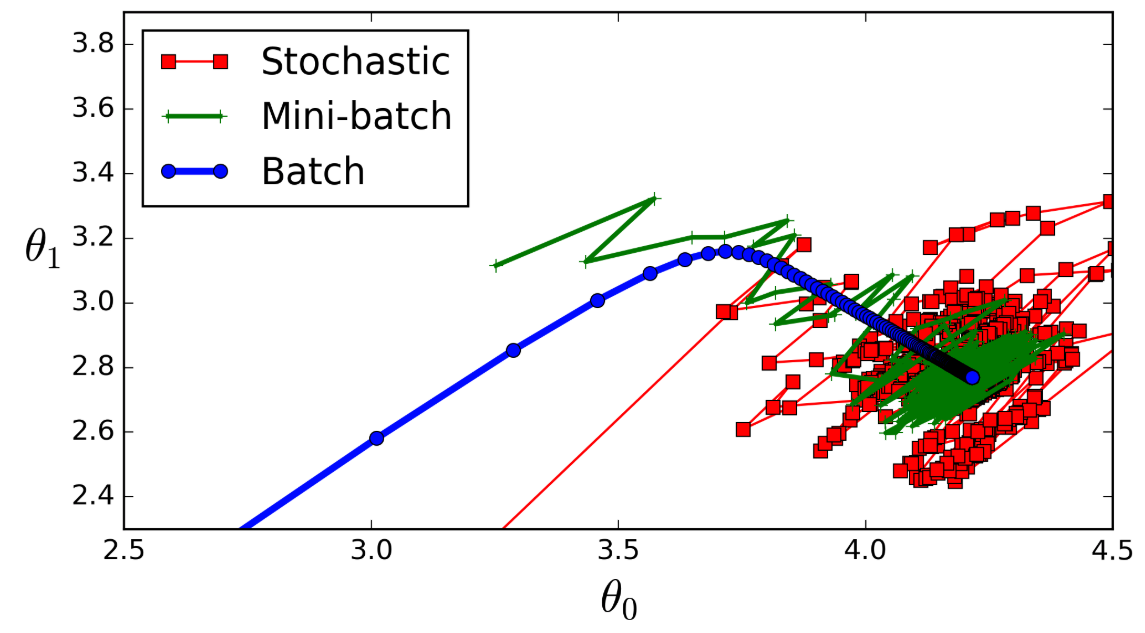
\includegraphics[width=\linewidth]{batch.png}
  \caption{Paths of Training in Different Batch Size \cite{sgd}}
  \label{BatchFig}
\end{figure}

\section{Training Result and Evaluation}
This section reports the result of the training with its specifications and the evaluation result of the trained model.
\subsection{Training Specification} 
\textbf{Batch Size} The batch is collection of a few samples of entire data that is propagated through the network for each step of iteration of training. Researchers and practitioners uses batch because of the following reasons: \\
\begin{displayquote}
1) \textbf{Training with batch requires less memory}\\
Since we train the network with fewer samples, the overall training procedure requires less memory. This is especially useful when the entire number data is massive which is well fit for deep learning.\\

2) \textbf{Typically networks train faster with using batch}\\This is because we update the weights "more" when using batch. For example, if we 100 entire data samples to train, if we use batch with size 10, it updates the weights for 10 times for one epoch\footnote{epoch is a unit term that refers to when an entire data set is passed both forward and backward through the neural network once.}, however, if we use all samples during propagation it makes only 1 update per one epoch.  
\end{displayquote}
However, there also exists a disadvantages of using batch. As a main disadvantage, the smaller the batch size, the estimate of the gradient becomes less accurate. For more visual explanation, one can see that the direction of the mini-batch (green) or stochastic (red; which equals to the case of batch size 1) fluctuates much more in comparison to the direction of the full batch (blue) in Figure \ref{BatchFig}, which plots the training paths to the global optimum with different size of batches.

Concluding the remarks about the batch training, one inevitably needs to use the batch because of the GPU memory limitation. Deep learning requires huge amount of data to achieve the fine performance and one can't train those all huge data at once with full-batch at real situation. Therefore, every researchers uses batch size, usually in range of 8 to 64 for the training of neural network. 

We had performed the training with the batch size 8. This size is determined considering the memory limitation of GPU memory 8GB. One might can enlarge this size up to 128 to shorten the time of training per epoch if memory permits.\\\\ 
\begin{figure}
  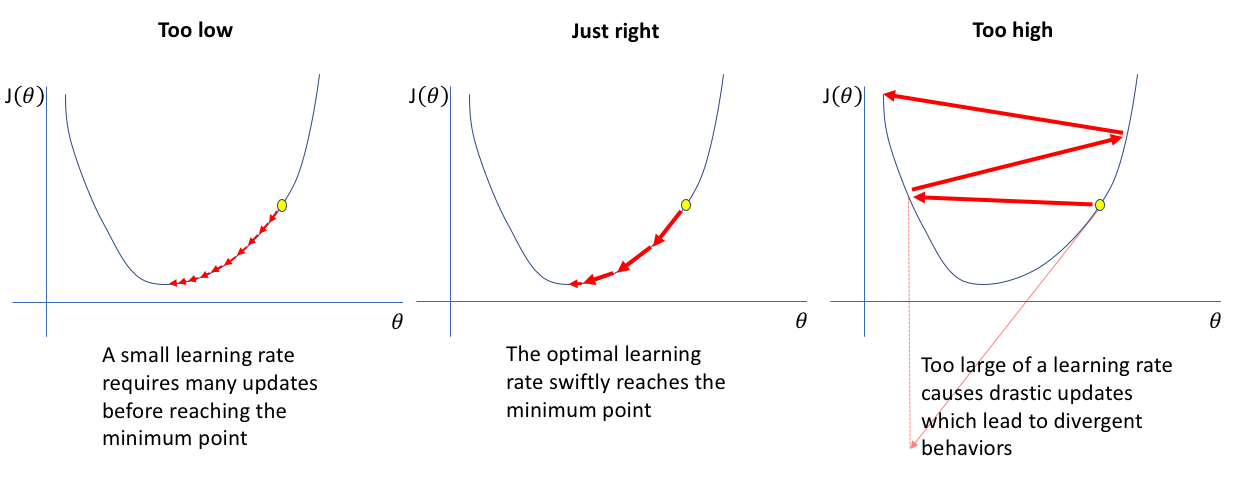
\includegraphics[width=\linewidth]{lr.png}
  \caption{Adequate Learning Rate Guarantees Stable Training \cite{lrExample}}
  \label{LrFig}
\end{figure}
\textbf{Learning Rate} Learning rate is a configurable hyper-parameter that controls how much we are adjusting the weights(or often called in another name, "nodes") of our network with respect the loss gradient. This can be explicitly explained as following:

\begin{gather*}
    \theta_{i+1} = \theta_{i} - \eta \frac{\partial}{\partial \theta_{i}} \\
    \text{where } \theta_{i} \text{ is one of elements in set of weights in step } i \text{ ,} \\ \theta_{i+1} \text{ is that of step } i+1 \text{and } \eta \text{ refers to learning rate} 
\end{gather*}\\
When training neural network, learning rate is important and needs to decay alongside the step increment. This is because if learning rate is too high, neural network can achieve its local optimum, however if it's too low, the entire training takes too much time to get to the optimum. This is illustrated in Figure \ref{LrFig}. 

This research has adopted learning rate of 0.01 with decay rate 0.95 for every 5000 training step. This learning rate and its decay rate configuration is adopted which results in the most fast and stable training after a few experiments with different learning rate and decay rate. As like any other deep learning model configuration, there may exist better configuration of learning rate and decay rate for the model we had used. \\\\
\textbf{Sequence Padding} Sequence padding is the process to make all inputs to have the same length with pseudo vector since a neural network expects the same length of input. 

This research has adopted two different padding sizes, 35842 and 20158, one for the input type of government measure description, another for the input type of article content respectively. Those numbers are determined by the maximal input size of each type of input. In addition to the padding size, this research adopted "post" padding which pads the pseudo vector to the back of the original sentence.\\\\

\begin{figure}
  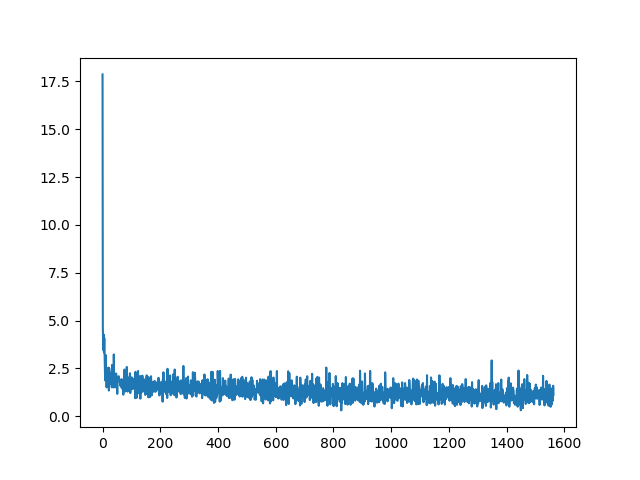
\includegraphics[width=1.1\linewidth]{trainLoss.png}
  \caption{Train Loss}
  \label{trainFig}
\end{figure}

\begin{figure}
  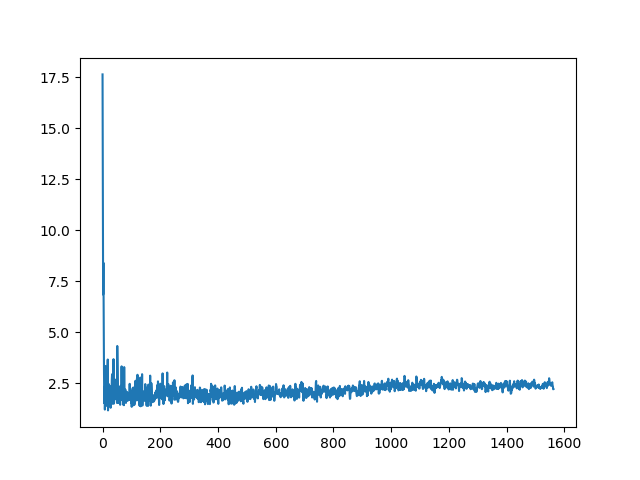
\includegraphics[width=1.1\linewidth]{testLoss.png}
  \caption{Test Loss}
  \label{testFig}
\end{figure}

\begin{figure}
  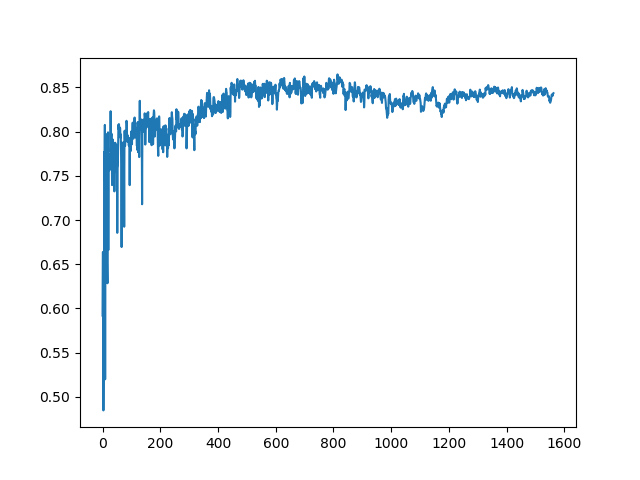
\includegraphics[width=1.1\linewidth]{aucroc.png}
  \caption{Increment of AUC-ROC while training}
  \label{aucrocFig}
\end{figure}
\subsection{Training Result}
\textbf{Train/Test Loss} Training loss converges to around \(1.25\) after 80,000 iteration step of training which corresponds to \(8.7\) epochs. The loss plot of training data is shown in Figure \ref{trainFig}. Test loss converges to around \(2\) after 100,000 iteration step of training which corresponds to \(10.9\) epochs. The loss plot of test data is shown in Figure \ref{testFig}. Both train and test loss is logged and plotted every 100 iteration of training step with batch size \(8\), which corresponds to 0.087 epoch. \\\\
\begin{figure}
  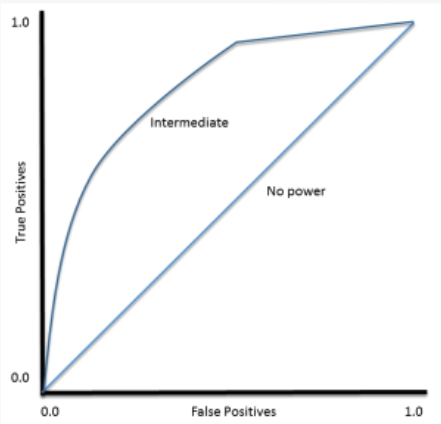
\includegraphics[width=0.8\linewidth]{aucrocarea.png}
  \caption{Area Under Curve of Receiver-Operating Characteristic \cite{aucrocplot}}
  \label{aucrefFig}
\end{figure}\textbf{AUC-ROC Evaluation} The model achieved the highest AUC-ROC metric \(0.86\) at 800,000 iteration step of training and keep maintaining its AUC-ROC metric over \(0.825\) after \(80,000\) iteration step of training. 

The AUC-ROC curve is a performance measurement for classification problem at various thresholds settings. Since the model accuracy varies upon the which thresholds settings being selected, one needs to consider every case of thresholds together to measure the model's classification power conclusively. 

The ROC at a certain threshold is defined as following:
\begin{gather*}
    \text{ROC} (t) = \frac{\text{TPR (True Positive Rate)}}{\text{FPR (False Positive Rate)}}\\\\
    \text{where } \text{TPR} = \frac{\text{TP (True Positive)}}{\text{TP (True Positive) + FN (False Negative)}}\\
    \text{FPR} = \frac{\text{FP (False Positive)}}{\text{FP (False Positive) + TN (True Negative)}}
\end{gather*}\\
It intuitively refers to that how many correct answer has the model provided compared to the incorrect answers. 

As mentioned earlier, AUC means "Area Under Curve". ROC for every case of t has calculated and plotted as like shown in  Figure \ref{aucrefFig}

The maximum value of the AUC-ROC is 1 which means that the model always classifies the correct label. Our model scored 0.85 of AUC-ROC which provides the correct label regarding whether a certain article is citable or not for given specific government measure description with the probability of 85\%.\\\\
\section{Conclusion}
\subsection{Main Contribution}\\
The research has made off-the-shelf public dataset in the field of law. Then the research has proposed the novel neural network structure that can process legal article contents and government measure description seperately and then merge and feed those two into one legal reasoning network. This kind of network architecture has successfully learned whether a legal article can be cited or not for given government description with 85\% of accuracy in terms of AUC-ROC metric.


This research has proved that the human-able task, which is to determine whether a given article content is citable or not for the given textual description, is also successfully learnable by artificial intelligence. Moreover, compared to the human legal reasoning process which is only able to subjectively understand how much certain article content could be cited, neural network can numerically show how much a legal article is citable with probability. This objective and numeric manner of representation may assist human legal practitioners to list up which legal articles are most-citable or must-cite articles in their working process. This kind of numerical objectivity is especially important for lowering the communication cost between groups of legal practitioners since it can provide an objective language for legal discussion and facilitate the speed of the discussion until it gets to the specific agreement which articles must be dealt in high priority.  


Moreover, this research has published the reproducible code in Github Page (Please refer to the \textit{Appendix C: Github Page)} which is publicly accessible via online so that everyone can verify the result explained in this research with pre-trained weight that is used in this research and customize the codes for the future research development.



\subsection{Further Research Point}\\
This research has proven that the deep learning approach is successfully working for the field of law. However, according to the anonymous commentator who's working as an attorney in South Korean law firm, this successful result is mainly due to the well-refined input that is already cleared from the messy raw documents by lots of lawyers with tremendous effort being invested. In other words, the "Factual Aspect" given by WTO panel report has already been well-cleared data, thus the successful result of this research might be mainly due to those human labor intensive clearing effort. Therefore, the Artificial Intelligence that really aims to develop the legal field might have to focus on how to clear the raw data with less effort rather than focusing on the replacing the legal reasoning or legal judgment.

% references
\bibliographystyle{ACM-Reference-Format}
\bibliography{deepWTO}

\begin{appendices}
\section*{Appendix A : Dispute Settlements}
This section denotes the dispute settlement ID that has a Panel or Appellate Body report.
\begin{lstlisting}[breaklines, language=yaml, frame=tlrb]
Panel:
  #dispute settlement id which has panel report
  ds_numb: [2, 7, 8, 10, 11, 12, 14, 18, 22, 24, 31, 33, 34, 46, 50, 56, 58,
            60, 62, 67, 68, 69, 70, 72, 75, 76, 79, 84, 87, 90, 98, 99, 103,
            108, 110, 113, 114, 121, 122, 126, 132, 135, 136, 138, 139, 141,
            142, 146, 152, 155, 156, 161, 162, 163, 165, 166, 169, 170, 174,
            175, 177, 178, 184, 189, 192, 202, 204, 207, 212, 213, 217, 219,
            221, 231, 234, 238, 243, 244, 245, 246, 248, 249, 251, 252, 253,
            254, 257, 258, 259, 264, 265, 266,267, 268, 269, 276, 282, 283,
            285, 286, 290, 294, 295, 296, 301, 302, 308, 312, 315, 316, 320,
            321, 322, 323, 332, 336, 339, 340, 342, 343, 344, 345, 350, 353,
            360, 363, 366, 367, 371, 379, 381, 384, 386, 391, 392, 394, 395,
            396, 397, 398, 399, 400, 401, 403, 406, 412, 413, 414, 415, 416,
            417, 418, 422, 425, 426, 427, 429, 430, 431, 432, 433, 435, 436,
            437, 438, 440, 441, 442, 444, 445, 447, 449, 453, 454, 456, 457,
            458, 460, 461, 464, 467, 468, 471, 472, 473, 475, 476, 477, 478,
            479, 480, 482, 483, 484, 485, 486, 487, 488, 490, 491, 492, 493,
            495, 496, 497, 499, 504, 505, 513, 518, 523, 526]

AppellateBody:
  #dispute settlement id which has AppellateBody report
  ds_numb: [2, 8, 10, 11, 18, 22, 24, 31, 33, 34, 46, 50, 56, 58, 60, 62,
           67, 68, 69, 70, 75, 84, 87, 90, 98, 103, 108, 110, 113, 121, 122,
           135, 136, 138, 139, 141, 142, 146, 161, 162, 165, 166, 169, 170,
           175, 177, 178, 184, 192, 202, 207, 212, 213, 217, 219, 231,
           234, 244, 245, 246, 248, 249, 251, 252, 253, 254, 257, 258,
           259, 264, 265, 266, 267, 268, 269, 276, 282, 283, 285, 286,
           294, 295, 296, 302, 308, 315, 316, 320, 321, 322, 332, 336,
           339, 340, 342, 343, 344, 345, 350, 353, 360, 363, 367, 371,
           379, 381, 384, 386, 394, 395, 396, 397, 398, 399, 400, 401,
           403, 406, 412, 414, 426, 429, 430, 431, 432, 433, 436, 437,
           438, 442, 444, 445, 449, 453, 454, 456, 457, 460, 461, 464,
           471, 472, 473, 475, 477, 478, 479, 486, 487, 490, 496, 497]

# Disputes that are handled under the same AppellateBody - legal basis refers to the DSU Art.9.1
LinkedAppellate: [{8, 10, 11}, {12, 14}, {67, 68, 62}, {75, 84}, {110, 87},
                  {113, 103}, {139, 142}, {146, 175}, {169, 161}, {177,178},
                  {217, 234}, {258, 259, 248, 249, 251, 252, 253, 254},
                  {339, 340, 342}, {384, 386}, {394, 395, 398}, {403, 396},
                  {400, 401}, {416, 417, 418, 415}, {426, 412},
                  {432, 433, 431}, {441, 435}, {444, 445, 438}, {458, 435},
                  {460, 454}, {467, 435}, {477, 478}, {496, 490}, {472, 497}]

\end{lstlisting}


\section*{Appendix  B : TextCNN & Legal Reasoning Network \label{codeblock_model}} This section introduces the code block to implement the TextCNN \& Legal Reasoning network [ \ref{fig:teaser}] used in this research.\\\\
\textbf{The Highest Wrapper Block}
\begin{lstlisting}[breaklines, language=Python, frame=tlrb]
# -*- coding:utf-8 -*-
__author__ = 'Randolph'
__modify__ = 'Zachary'

import tensorflow as tf
from utils.layers import do_cnn, fc_w_nl_bn


class OneLabelTextCNN(object):
    """A CNN for generation of text-seq encoding."""

    def __init__(self,
                 sequence_length_gov,
                 sequence_length_art,
                 vocab_size,
                 fc_hidden_size,
                 embedding_size,
                 embedding_type,
                 filter_sizes,
                 num_filters,
                 l2_reg_lambda=0.0,
                 pretrained_embedding=None):

        # Placeholders for input, output, dropout_prob and training_tag
        self.input_x_gov = 
        tf.placeholder(tf.int32,
                      [None, sequence_length_gov],
                      name="input_x_gov")

        self.input_x_art = 
        tf.placeholder(tf.int32,
                      [None, sequence_length_art],
                      name="input_x_art")

        self.input_y = 
        tf.placeholder(tf.float32,
                      [None, 1],
                      name="input_y")

        self.dropout_keep_prob = 
        tf.placeholder(tf.float32,
                    name="dropout_keep_prob")

        self.is_training = 
        tf.placeholder(tf.bool,
                      name="is_training")

        self.global_step = 
        tf.Variable(0,
                   trainable=False,
                   name="Global_Step")

        # Embedding Layer
        with tf.device("/cpu:0"), tf.name_scope("embedding"):
            # Use random generated the word vector by default
            # Can also be obtained through our own word vectors trained
            # by our corpus
            if pretrained_embedding is None:
                self.embedding = tf.Variable(tf.random_uniform(
                    [vocab_size,
                     embedding_size],
                    minval=-1.0,
                    maxval=1.0,
                    dtype=tf.float32),
                    trainable=True,
                    name="embedding")
            else:
                if embedding_type == 0:
            self.embedding = tf.constant(pretrained_embedding,
                        dtype=tf.float32,
                        name="embedding")
                if embedding_type == 1:
            self.embedding = tf.Variable(pretrained_embedding,
                        trainable=True,
                        dtype=tf.float32,
                        name="embedding")
            self.embedded_sentence_gov = tf.nn.embedding_lookup(
                self.embedding,
                self.input_x_gov)

            self.embedded_sentence_art = tf.nn.embedding_lookup(
                self.embedding,
                self.input_x_art)

            self.embedded_sentence_expanded_gov = tf.expand_dims(
                self.embedded_sentence_gov, axis=-1)

            self.embedded_sentence_expanded_art = tf.expand_dims(
                self.embedded_sentence_art, axis=-1)

        # h_drop_gov_args = filter_sizes, embedding_size, num_filters

        h_drop_gov = 
        do_cnn(gov_or_art="gov",
        filter_sizes=filter_sizes,
        embedding_size=embedding_size,
        num_filters=num_filters,
        embedded_sentence_expanded=
        self.embedded_sentence_expanded_gov,
        is_training=self.is_training,
        sequence_length=sequence_length_gov,
        fc_hidden_size=fc_hidden_size,
        dropout_keep_prob=self.dropout_keep_prob)

        h_drop_art = 
        do_cnn(gov_or_art="art",
        filter_sizes=filter_sizes,
        embedding_size=embedding_size,
        num_filters=num_filters,
        embedded_sentence_expanded=
        self.embedded_sentence_expanded_art,
        is_training=self.is_training,
        sequence_length=sequence_length_art,
        fc_hidden_size=fc_hidden_size,
        dropout_keep_prob=self.dropout_keep_prob)


        self.h_drop = 
        tf.concat(values=[h_drop_gov,
                          h_drop_art], axis=1)

        self.legal = 
        fc_w_nl_bn("legal",
                    fc_hidden_size=2 * fc_hidden_size,
                    input_tensor=self.h_drop,
                    output_size=fc_hidden_size,
                    is_training=self.is_training)

        # Final scores
        with tf.name_scope("output"):
            W = tf.Variable(
            tf.truncated_normal(
                shape=[fc_hidden_size, 1], 
                stddev=0.1,
                dtype=tf.float32),
                name="W")
            b = tf.Variable(
                tf.constant(value=0.1,
                shape=[1],
                dtype=tf.float32),
                name="b")
            self.logits = 
                tf.nn.xw_plus_b(
                self.legal, W, b,
                name="logits")
            self.scores = 
                tf.sigmoid(self.logits,
                           name="scores")

        # Calculate mean cross-entropy loss, L2 loss
        with tf.name_scope("loss"):
        losses =
        tf.nn.weighted_cross_entropy_with_logits(
            targets=self.input_y,
            logits=self.logits,
            pos_weight=26.303)

        losses = 
        tf.reduce_mean(
            tf.reduce_sum(losses, axis=1),
                          name="sigmoid_losses")
        l2_losses = 
            tf.add_n([tf.nn.l2_loss(tf.cast(v,                             tf.float32))
            for v in tf.trainable_variables()],
            name="l2_losses") * l2_reg_lambda
        self.loss = tf.add(losses, l2_losses, name="loss")
\end{lstlisting}
\textbf{TextCNN Block}
\begin{lstlisting}[language=Python, frame=tlrb]
def do_cnn(gov_or_art,
           filter_sizes,
           embedding_size,
           num_filters,
           embedded_sentence_expanded,
           is_training,
           sequence_length,
           fc_hidden_size,
           dropout_keep_prob):
    # Create a convolution 
    # and maxpool layer for each filter size
    
    pooled_outputs = []
    
    for filter_size in filter_sizes:
        with tf.name_scope(
        "conv-filter{}_{}".format(
            filter_size,
            gov_or_art)):
            
            # Convolution Layer
            filter_shape = [filter_size,
                            embedding_size,
                            1,
                            num_filters]
            W = tf.Variable(
                    tf.truncated_normal(
                        shape=filter_shape, 
                        stddev=0.1, 
                        dtype=tf.float32),
                        name="W")
                  
            b = tf.Variable(
                    tf.constant(
                        value=0.1,
                        shape=[num_filters],
                        dtype=tf.float32),
                        name="b")
            conv = tf.nn.conv2d(
                embedded_sentence_expanded,
                W,
                strides=[1, 1, 1, 1],
                padding="VALID",
                name="conv")
            
            conv = tf.nn.bias_add(conv, b)
            
            # Batch Normalization Layer
            conv_bn =
            tf.layers.batch_normalization(
                conv,
                training=is_training)
            
            # Apply nonlinearity
            conv_out = tf.nn.relu(
                        conv_bn,
                        name="relu")
        
        with tf.name_scope(
        "pool-filter{}_{}".format(
            filter_size,
            gov_or_art)):
            
            # Maxpooling over the outputs
            pooled = tf.nn.max_pool(
                conv_out,
                ksize=
                [1, 
                sequence_length 
                - filter_size + 1, 
                1, 1],
                strides=[1, 1, 1, 1],
                padding="VALID",
                name="pool")
        
        pooled_outputs.append(pooled)
    
    # Combine all the pooled features
    num_filters_total = 
        num_filters * len(filter_sizes)
    pool = tf.concat(pooled_outputs,
                     axis=3)
    pool_flat = tf.reshape(pool,
        shape=[-1, num_filters_total])
    
    # Fully Connected Layer
    with tf.name_scope(
    "fc_{}".format(gov_or_art)):
        W = tf.Variable(
            tf.truncated_normal(
                shape=[num_filters_total,
                       fc_hidden_size],
                       stddev=0.1,
                       dtype=tf.float32),
                       name="W")
        b = tf.Variable(
            tf.constant(value=0.1,
                    shape=[fc_hidden_size],
                        dtype=tf.float32),
                        name="b")
        fc = tf.nn.xw_plus_b(pool_flat, W, b)
        
        # Batch Normalization Layer
        fc_bn = tf.layers.batch_normalization(
        fc, training=is_training)
        
        # Apply nonlinearity
        fc_out = tf.nn.relu(fc_bn,
                            name="relu")
    
    # Highway Layer
    with tf.name_scope(
    "highway_{}".format(gov_or_art)):
        highway = highway_layer(
        fc_out,
        fc_out.get_shape()[1],
        gov_or_art=gov_or_art,
        num_layers=1,
        bias=0)
    
    # Add dropout
    with tf.name_scope(
    "dropout_{}".format(gov_or_art)):
        h_drop = tf.nn.dropout(
            highway,
            dropout_keep_prob)
    return h_drop
\end{lstlisting}
\textbf{FC layer}
\begin{lstlisting}[language=Python, frame=tlrb]
def fc_w_nl_bn(name_scope,
               fc_hidden_size,
               input_tensor,
               output_size,
               is_training):
    # Fully Connected Layer
    with tf.name_scope(name_scope):
        W = tf.Variable(
            tf.truncated_normal(
            shape=[fc_hidden_size,
                   output_size],
                   stddev=0.1,
                   dtype=tf.float32),
            name="W")
        b = tf.Variable(
            tf.constant(value=0.1,
                        shape=[output_size],
                        dtype=tf.float32),
            name="b")
        fc = tf.nn.xw_plus_b(
            input_tensor,
            W,
            b)
        
        # Batch Normalization Layer
        fc_bn = 
        tf.layers.batch_normalization(
            fc,
            training=is_training)
        
        # Apply nonlinearity
        fc_out = tf.nn.relu(fc_bn,
                            name="relu")
        return fc_out

\end{lstlisting}
\section*{Appendix C : Github Page}
Every code line used to prepare the dataset and train/test the model is included in the following url:
\begin{displayquote}
\hyperlink{https://github.com/syyunn/DeepWTO}{https://github.com/syyunn/DeepWTO}
\end{displayquote}\\\\
Follwing pages include the README.md file that you can locate at the above link.
\end{appendices}
\end{document}
